
%(BEGIN_QUESTION)
% Copyright 2010, Tony R. Kuphaldt, released under the Creative Commons Attribution License (v 1.0)
% This means you may do almost anything with this work of mine, so long as you give me proper credit

\noindent
{\bf Laboratorieøvelse}

\vskip 5pt

Oppgaven deres er å bygge, kalibrere og dokumentere et pneumatisk system bestående av en pneumatisk sløyferegulator koblet til en reguleringsventil. Hvis gruppens prosessregulator ikke har PV- og/eller SP-indikatorer som kan kalibreres og justeres inn, må dere bygge en fungerende prosess som regulatoren kan styre.

Et ekstra mål i denne laben er å kappe, bøye og tilpasse instrumentrør i metall på riktig måte. Hver student skal bøye et stykke kobber- eller rustfritt instrumentrør et sted i regulator-/ventilsystemet og vise instruktøren at rørene passer pent (rette hjørner, riktige offset, i vater og lodd). Bøying av instrumentrør er i stor grad et håndverk, og krever øvelse for å mestres.

Tabellen under viser målene du og gruppen må fullføre innen tiden som er satt av til denne øvelsen. Merk at noen mål er individuelle, mens andre gjelder gruppen som helhet:

\underbar{Tabell for måloppnåelse:}

% No blank lines allowed between lines of an \halign structure!
% I use comments (%) instead, so that TeX doesn't choke.

$$\vbox{\offinterlineskip
\halign{\strut
\vrule \quad\hfil # \ \hfil & 
\vrule \quad\hfil # \ \hfil & 
\vrule \quad\hfil # \ \hfil & 
\vrule \quad\hfil # \ \hfil & 
\vrule \quad\hfil # \ \hfil & 
\vrule \quad\hfil # \ \hfil & 
\vrule \quad\hfil # \ \hfil \vrule \cr
\noalign{\hrule}
%
% First row
{\bf Prestasjonsmål} & {\bf Vurdering} & {\bf 1} & {\bf 2} & {\bf 3} & {\bf 4} & {\bf Gruppe} \cr
%
\noalign{\hrule}
%
% Another row
Prototypeskisse ({\it før systemet bygges!}) & mestring & -- & -- & -- & -- & \cr
%
\noalign{\hrule}
%
% Another row
Endelig sløyfediagram og systeminspeksjon & mestring & & & & & -- -- -- -- \cr
%
\noalign{\hrule}
%
% Another row
Indikatorkalibrering / fungerende prosess & mestring & -- & -- & -- & -- &  \cr
%
\noalign{\hrule}
%
% Another row
Demonstrasjon av direkte og omvendt virkning & mestring & -- & -- & -- & -- &  \cr
%
\noalign{\hrule}
%
% Another row
Forklar proporsjonal reguleringsmekanisme & mestring & & & & & -- -- -- -- \cr
%
\noalign{\hrule}
%
% Another row
Metallrør korrekt tilpasset & mestring & & & & & -- -- -- -- \cr
%
\noalign{\hrule}
%
% Another row
Labspørsmål: Utvalg/testing & proporsjonal &  &  &  &  & -- -- -- -- \cr
%
\noalign{\hrule}
%
% Another row
Labspørsmål: Idriftsettelse & proporsjonal &  &  &  &  & -- -- -- -- \cr
%
\noalign{\hrule}
%
% Another row
Labspørsmål: Hoderegning & proporsjonal &  &  &  &  & -- -- -- -- \cr
%
\noalign{\hrule}
%
% Another row
Labspørsmål: Diagnostikk & proporsjonal &  &  &  &  & -- -- -- -- \cr
%
\noalign{\hrule}
%
% Another row
Nedstenging og opprydding i lab & mestring & -- & -- & -- & -- &  \cr
%
\noalign{\hrule}
} % End of \halign 
}$$ % End of \vbox

Den eneste ``proporsjonale'' vurderingen i denne aktiviteten er labspørsmålene, som besvares individuelt av hver student. En liste over mulige labspørsmål finnes på slutten av dette arket. Labspørsmålene er ment å styre laboratoriearbeidet like mye som å måle forståelse, og instruktøren kan derfor stille disse spørsmålene dag for dag i stedet for samlet på én dag.

\vskip 10pt

{\bf Det er avgjørende at gruppen planlegger hva som skal fullføres hver dag. Et kort gruppemøte (10 minutter) i starten av hver labøkt er en god måte å gjøre dette på: gå gjennom hva som er gjort, hva som gjenstår, og hvilke vurderinger dere bør være klare for. Det er mye arbeid med å bygge, dokumentere og feilsøke fungerende instrumentsystemer!}

Når dere jobber med systemet, vil dere uunngåelig møte problemer. Forsøk alltid å løse problemene som gruppe før dere ber om hjelp fra instruktør. Hvis dere fortsatt trenger hjelp, skriv gruppens farge på labtavlen sammen med en kort beskrivelse av hva dere trenger hjelp til. Instruktøren hjelper gruppene i den rekkefølgen de står oppført på tavlen.

$$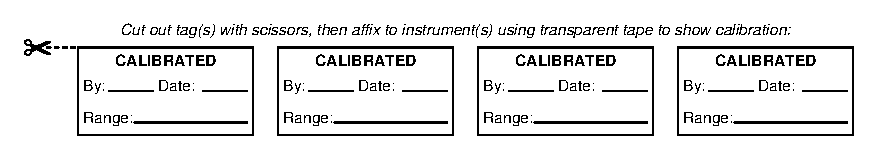
\includegraphics[width=15.5cm]{i01495x01.eps}$$





\vfil \eject

\noindent
{\bf Laboratorieøvelse -- valg av komponenter og systemplanlegging}

\vskip 5pt

Et av de vanligste problemene studenter møter når de bygger fungerende systemer, enten det er en krets på koblingsbrett eller en instrumentsløyfe gjennom et helt rom, er riktig sammenkobling og konfigurering av alle komponenter. En uheldig tendens er å bare begynne å koble sammen deler og i praksis designe systemet underveis. Dette fører ofte til feilkoblinger og systemer som ikke fungerer, og kan i verste fall skade komponenter.

En bedre tilnærming er å planlegge på forhånd ved å designe systemet før bygging. Dette gjøres enkelt ved å lage en skisse som viser hvordan alle komponentene skal kobles sammen, deretter analysere skissen og gjøre endringer før noe bygges. Gjort som gruppe sikrer dette at alle forstår hvordan systemet skal virke og monteres. ``Prototype''-skissen trenger ikke være ekstremt detaljert, men den må være tydelig nok til at man ser hvilke terminaler (og porter) som kobles til hva. For eksempel skal den være tydelig nok til at alle DC-komponenter får riktig polaritet. Hvis systemet inneholder mye rørføring (rør/slanger), bør dette også vises.

\vskip 10pt

Første steg er å velge både reguleringsventil og pneumatisk regulator som skal brukes. Siden dette er et helt {\it pneumatisk} system, trengs verken I/P-omformer eller elektronisk ventilposisjoner. Regulatorens utgangslinje kobles enten direkte til ventilens membranaktuator eller til signalinngangen på en pneumatisk posisjoner. Hvis regulatoren har PV- og SP-indikatorer, anbefales en stor reguleringsventil, for eksempel Fisher E-body i laben. Hvis regulatoren {\it ikke} har PV-/SP-indikator for kalibrering, bør dere velge en liten reguleringsventil (for eksempel Research Control) og bygge en fungerende trykkprosess, siden dette blir erstatningen for kalibrering av PV/SP-indikatorer.

Neste steg er å finne relevant dokumentasjon for regulatoren. Nesten alle instrumenter i laben har elektronisk dokumentasjon på produsentens nettsider, så internett (og/eller Instrumentation Reference, der mange manualer allerede er samlet) er beste ressurs. Bruk dokumentasjonen til å finne riktig installasjon, rørtilkobling og kalibrering av regulatoren. Instruktøren vil kontrollere at dere har funnet og forstått manualene.

Etter at egnet regulator og dokumentasjon er funnet, bør regulatoren testes kvalitativt før den monteres i systemet. Dette innebærer å legge på et pneumatisk signal på PV-inngangen i automatisk modus og kontrollere at pneumatisk utgang varierer når inngangen varieres. Hvis regulatoren ikke svarer riktig, varsle instruktøren og merk regulatoren med en lapp som beskriver hva den gjør (eller ikke gjør). Testen bør utføres med ``integral'' og ``derivative'' (hvis tilgjengelig) satt til minimum. For derivative betyr dette null minutter. For integral betyr dette maksimalt antall minutter per repetisjon (eller minimum repetisjoner per minutt).

\vskip 10pt

Gruppens prototypeskisse er så viktig at instruktøren krever at planen foreligger før bygging starter. {\it En gruppe som begynner bygging uten verifisert plan vil bli stoppet og får ikke fortsette før prototypeplan er laget og godkjent!} Hvert gruppemedlem skal ha enkel tilgang til planen (helst egen kopi) gjennom hele byggeprosessen. Prototypetegning er både en ferdighet og en arbeidsvane som bør utvikles i skolen og tas med inn i yrkeslivet.

\vskip 10pt

{\bf Planlegging av et fungerende system bør ikke ta mer enn en time dersom gruppen jobber effektivt, og kan spare mange timer frustrasjon (og mulig komponentskade!).}




\vfil \eject

\noindent
{\bf Laboratorieøvelse -- bygging av systemet}

\vskip 5pt

Instrumenteringslaben er satt opp for å gjøre det enkelt å bygge fungerende pneumatiske instrumentsløyfer, med panel for pneumatisk regulator og ``racker'' med 2-tommers vertikale rør for montering av feltmonterte pneumatiske regulatorer (f.eks. Fisher MultiTrol, Foxboro 43).

Når prototypeskissen er godkjent av instruktøren, kan dere starte byggingen. Den pneumatiske regulatoren kan være forhåndsmontert i panel, eller være en feltmontert regulator som festes til 2-tommers rør med spesialbrakett og U-bolter. Disse finnes i instrumentlageret.

Til slutt må det pneumatiske systemet få et sløyfenummer, slik at alle instrumenter kan merkes riktig. Sløyfenummeret må være unikt slik at ingen annen gruppe merker instrumenter og kabler likt. En måte å sikre unikt nummer på er å bruke motstandsfargekodens tallverdi for gruppens farge. Er dere for eksempel ``Rød'' gruppe, kan sløyfenummeret være ``2''.

\vskip 10pt

{\bf Vanlige feil:}

\begin{itemize}
\item{} Manglende bruk av produsentdokumentasjon for feltinstrumenter (f.eks. hvordan de kobles med rør, hvordan de kalibreres).
\item{} Feltinstrument(er) monteres i upraktiske posisjoner slik at tilkoblinger eller deksler blir vanskelige å nå.
\item{} Feil montering av rør-/slangefittings (for eksempel forsøk på å skru slangefittings i rørgjenger og omvendt).
\item{} Studenter jobber isolert på hver sin del av systemet uten å dele hva som er gjort og hvordan. Hele gruppen må lære alle deler av systemet.
\end{itemize}

\vskip 10pt

{\bf Bygging av et fungerende system bør ikke ta mer enn én full labøkt (3 timer) dersom alle komponenter er tilgjengelige og gruppen jobber effektivt!}




\vfil \eject

\noindent
{\bf Laboratorieøvelse -- dokumentasjon av systemet}

\vskip 5pt

Hver student skal lage sitt eget {\it sløyfediagram} for gruppens system, etter ISA-konvensjoner. Eksempler vises i neste oppgave i dette arket. Sløyfediagrammene skal være {\it komplette} og {\it detaljerte}, og vise alle rørtilkoblinger, alle signallinjer, alle fittings, områder/rangepunkter osv. Prinsippet er at diagrammet skal være så tydelig at enhver kan følge det og se hva som er koblet til hva, også personer uten instrumentbakgrunn. I industrien bygges sløyfer ofte av kontraktører med begrenset systemforståelse. Diagrammene de jobber etter må derfor være så detaljerte at korrekt sammenkobling er mulig uten full forståelse av funksjonen.

Alle instrumenter og alle rør/slanger i sløyfen skal merkes med ISA-standard tagnummer. En enkel metode er å bruke korte biter maskeringstape på hver kabel (og hvert instrument) og skrive med permanent tusj. Selv om det ikke finnes én bransjestandard for merking av signalkabler, er en god praksis å merke hver tokjernerskabel med tagnummeret til feltinstrumentet den går til. Dermed bør alle kabellengder i en trykktransmitterkrets merkes ``PT-$x$'' (der ``$x$'' er sløyfenummer), alle strømningsventiler ``FV-$x$'', osv. Husk at hele sløyfen defineres av prosessvariabelen den måler: hvis PV er {\it temperatur}, blir transmitteren {\it T}T, reguleringsventilen {\it T}V, regulatoren {\it T}C osv.

Når hele gruppen er ferdig med individuelle sløyfediagrammer, tilkall instruktør for sløyfeinspeksjon. Da får studentene på omgang forklare hele sløyfen, mens de andre samtidig kontrollerer diagrammene for feil og mangler. Instruktøren inspiserer også installasjonskvalitet, med fokus på for eksempel oppfliset ledning, dårlig krymping av terminaler, dårlig kabelføring, manglende merking, manglende lokk på ledningskanaler osv. Gruppen må rette alle avvik for å få godkjent systemet.

Etter godkjent inspeksjon skal hvert gruppemedlem legge sløyfediagrammet i diagramholderen midt i laben bak hovedpanelet. Når dere senere skal feilsøke et annet gruppesystem, er dette stedet dere henter diagrammet fra.

\vskip 10pt

{\bf Vanlige feil:}

\begin{itemize}
\item{} Glemmer å merke alle signalrør/slanger (se eksempel på sløyfediagram).
\item{} Glemmer å merke alle feltinstrumenter med eget tagnavn (f.eks. PC-83).
\item{} Glemmer å notere alle portmerkinger for pneumatisk signal på regulator og ventil.
\item{} Glemmer å skrive navn på sløyfediagrammet.
\item{} Basere eget diagram på en lagkamerats diagram i stedet for å inspisere systemet selv.
\item{} Tegner ikke instrumentene i riktig orientering i sløyfearket (feltinstrumenter til venstre, kontrollrominstrumenter til høyre).
\end{itemize}

\vskip 10pt

{\bf Utarbeiding og inspeksjon av korrekte sløyfediagrammer bør ikke ta mer enn én full labøkt (3 timer) dersom gruppen jobber effektivt!}




\vfil \eject

\noindent
{\bf Laboratorieøvelse -- indikering av regulatorens kalibrering}

\vskip 5pt

Hvis gruppens pneumatiske regulator er en {\it indikerende} regulator (har PV- og SP-indikatorer), må gruppen kalibrere begge indikatorene og utføre justering slik at regulatoren ikke ser feil når PV=SP gjennom hele området. Hvis regulatoren ikke viser PV, hopp over denne delen og gå til neste del, der dere skal bygge et trykkreguleringssystem som regulatoren kan styre.

Som i alle kalibreringsoppgaver må instrumentresponsen kontrolleres mot én eller flere {\it referanser}. I dette tilfellet er en {\it testmanometer} for standard pneumatisk område 3-15 PSI en god referanse. Referanseinstrumentet må selvsagt være mer nøyaktig enn instrumentet (regulatoren) som kalibreres, så et vanlig trykkmanometer er ikke godt nok. Påkrevd kalibreringsnøyaktighet for regulatorens PV-indikator er $\pm$ 1\%.

Vedlikeholdsmanualen for den pneumatiske regulatoren viser hvordan luftkilder og testmanometre kobles til regulatoren for kalibrering og justering.

\filbreak

Dokumenter nøyaktigheten til PV-indikatoren før og etter justering i tabellen under, ved fem punkter gjennom måleområdet. ``Påført'' signal er lufttrykket du legger på PV-inngangen med luftkilde og testmanometer, og ``Indikert'' signal er regulatorens PV-viser:

% No blank lines allowed between lines of an \halign structure!
% I use comments (%) instead, so that TeX doesn't choke.

$$\vbox{\offinterlineskip
\halign{\strut
\vrule \quad\hfil # \ \hfil & 
\vrule \quad\hfil # \ \hfil & 
\vrule \quad\hfil # \ \hfil \vrule \cr
\noalign{\hrule}
%
% First row
Påført signal & Indikert verdi (før) & Indikert verdi (etter) \cr
%
\noalign{\hrule}
%
% Another row
 &  & \cr
%
\noalign{\hrule}
%
% Another row
 &  & \cr
%
\noalign{\hrule}
%
% Another row
 &  & \cr
%
\noalign{\hrule}
%
% Another row
 &  & \cr
%
\noalign{\hrule}
%
% Another row
 &  & \cr
%
\noalign{\hrule}
} % End of \halign 
}$$ % End of \vbox

Når kalibreringen er ferdig, må dere sette på en kalibreringsetikett med område og dato. På første side av labøvelsen finnes etiketter som kan klippes ut og festes på transmitteren.

\vskip 10pt

{\bf Vanlige feil:}

\begin{itemize}
\item{} Følger ikke produsentens instruksjoner for kalibrering og justering av indikatorene.
\item{} Kontrollerer ikke trykkregulatorer nøye før tilkobling til luftkilde (f.eks. kobler luftforsyning til ``out''-port).
\item{} Feil montering av rør-/slangefittings (for eksempel forsøk på å skru slangefittings i rørgjenger og omvendt).
\item{} Glemmer å sette på kalibreringsetikett etter kalibrering.
\end{itemize}

\vskip 10pt

{\bf Kalibrering av regulatoren bør ikke ta mer enn én full labøkt (3 timer) dersom gruppen jobber effektivt!}



\vfil \eject

\noindent
{\bf Laboratorieøvelse -- bygging av et trykkreguleringssystem}

\vskip 5pt

Hvis gruppens pneumatiske regulator ikke har PV- eller SP-indikatorer som kan kalibreres og justeres, må dere bygge et reelt trykkreguleringssystem som regulatoren kan styre. Dette gjør labøvelsen rettferdig mellom ulike grupper og regulatormodeller, siden kalibrering/justering av PV/SP-indikatorer kan være tidkrevende.

\vskip 10pt

En enkel måte å bygge en reell prosess som er lett å regulere med pneumatisk sløyferegulator, er å bruke håndventiler og volumtanker for å lage et andrordens etterslepsystem, der trykket i tank nummer to kan leses direkte av regulatoren som et 3-15 PSI-signal:

$$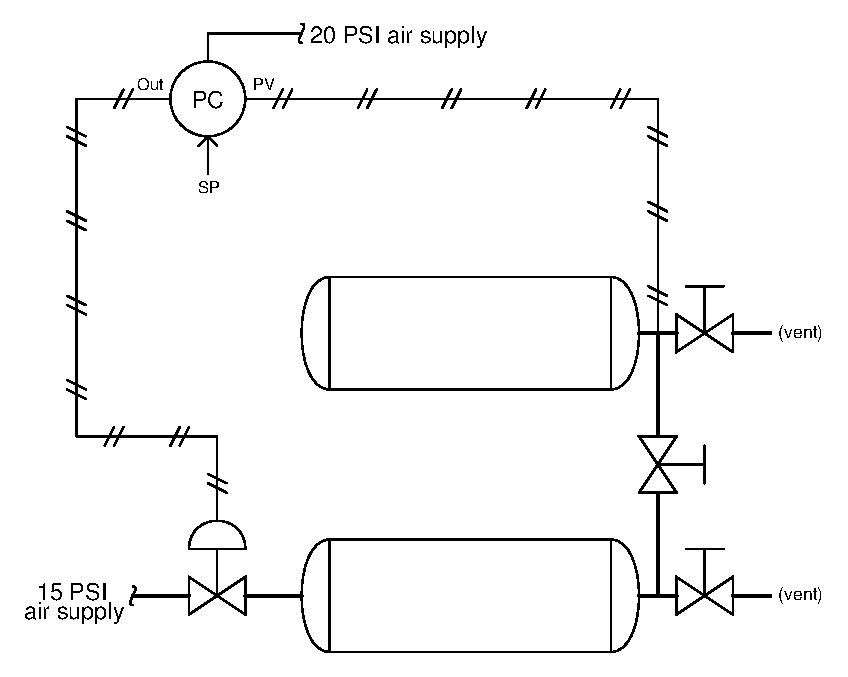
\includegraphics[width=15.5cm]{i01495x02.eps}$$

Nødvendig regulatorgain avhenger av størrelsen ($C_v$) på reguleringsventilen, tankvolumene og posisjonene til håndventilene. De to seriekoblede håndventilene endrer prosesstidskonstanter, mens de to avblødningsventilene fungerer som prosesslast. Store tankvolumer gir lange tidsforsinkelser, så unngå å koble for store volumtanker. Omtrent en halv gallon per tank fungerer godt. I en nødsituasjon holder det med én tank, men to tanker gir mer interessant reguleringsatferd.

For å gjøre den simulerte prosessen enda mer interessant kan dere koble en elektronisk trykktransmitter til PV-linjen og sende signalet til en enkel datalogger (eller skriverregistrator) for å registrere PV over tid mens dere justerer settpunkt, gain og prosessventiler.

\vskip 10pt

Demonstrasjon av stabil automatisk regulering vil vurderes som likeverdig med den kreditten andre grupper får ved kalibrering og justering av pneumatiske indikatorer.



\vfil \eject

\noindent
{\bf Laboratorieøvelse -- instrumentrør og fittings}

\vskip 5pt

Et tilleggsmål i denne laben er å lære riktig bøying av instrumentrør. Hver student skal bøye et stykke kobber- eller rustfritt rør et sted i regulator-/ventilsystemet og vise instruktøren at rørene passer pent (rette hjørner, korrekt offset, ingen gradvise bøyer, alle rette strekk i vater og lodd). Bøying av instrumentrør er et håndverk som krever trening.

Et ideelt sted å bruke rørbøying er linjene til og fra en ventilposisjoner, dersom ventilen bruker posisjoner. Hvis ikke, og dere bygger en fungerende prosess (for regulator uten PV/SP-indikering), kan dere bøye og tilpasse rør mellom prosesskar og andre deler av systemet.

Ruller med mykt kobberrør stilles til rådighet av instruktøren. Hver students rørstrekk bør være relativt kort (under 2 fot) for å begrense forbruk av rør. Regn med minst to forsøk før rørstrekket passer.

Videoer ligger på BTC Instrumentation sin YouTube-kanal og viser grunnleggende prosedyrer for kapping, bøying og montering av kompresjonsfittings. Hver gruppe har en profesjonell 1/4-tommers rørbøyer i skapet sitt som skal brukes i denne øvelsen.

Instrumentation Reference inneholder også manualer fra Swagelok og Parker som beskriver hvordan instrumentrørfittings fungerer, og hvordan rør tilpasses korrekt.

\vskip 10pt

{\bf Vanlige feil:}

\begin{itemize}
\item{} Bruk av teflontape eller annen tetning på gjenger i rørfittings (ikke nødvendig!).
\item{} Manglende teflontape eller annen tetning på rørgjenger for pipe fittings (nødvendig!).
\item{} Kaste brukte tube fittings etter jobben. Husk at selv om ferruler {\it ikke} kan gjenbrukes, kan muttere og fitting-kropper gjenbrukes.
\item{} Overstramming av kompresjonsfittings (ved {\it første} montering trengs bare 1-1/4 omdreining etter første kontakt). Ved remontering skal mutteren bare trekkes ``snug'', ikke swages på nytt med nye 1-1/4 omdreining.
\item{} Forsøk på å rette ut et rør som allerede er bøyd.
\end{itemize}





\vfil \eject

\noindent
{\bf Labspørsmål}

\vskip 5pt

\begin{itemize}
\item{} {\bf Valg og innledende testing}
\item{} Finn regulatorens restriksjon (orifice) og forklar formålet med den
\item{} Finn regulatorens klaff-/dyse-enhet og forklar formålet med den
\item{} Forklar trinn for trinn hvordan man sikrer en fungerende reguleringssløyfe for å kalibrere prosesstransmitteren uten å påvirke prosessen
\item{} Forklar trinn for trinn hvordan man sikrer en fungerende reguleringssløyfe for å stroketeste og kalibrere reguleringsventilen uten å påvirke prosessen
\item{} Identifiser foretrukket verktøyrekkefølge ved montering av tube fittings: fastnøkkel, ringnøkkel, tang, skiftenøkkel
\item{} Demonstrer korrekt bruk av håndluftpumpe som trykkilde for å simulere PV-signal inn til pneumatisk regulator
\end{itemize}

\filbreak

\begin{itemize}
\item{} {\bf Idriftsettelse og dokumentasjon}
\item{} Demonstrer hvordan potensiell farlig energi isoleres i systemet ({\it lock-out, tag-out}) og hvordan man verifiserer sikkert at energi faktisk er isolert før arbeid starter
\item{} Forklar hvordan en {\it tube fitting} tetter mot væskelekkasje
\item{} Forklar hvordan en konisk gjenget {\it pipe fitting} tetter mot væskelekkasje
\item{} Identifiser og forklar hvordan store signalvolumer i rør/slanger forringer ytelsen til pneumatiske instrumenter
\item{} Forklar hvordan regulatorens mekanisme for variabel gain virker, og demonstrer justering
\item{} Forklar og demonstrer hvordan regulatoren byttes mellom direkte og omvendt reguleringsmodus
\item{} Forklar hvordan regulatoren kan konfigureres for {\it av/på}-regulering (``bang-bang'')
\item{} Forklar hvor og hvordan PV og SP sammenlignes (subtraheres) i regulatormekanismen, siden alle proporsjonalregulatorer reagerer på {\it forskjellen} mellom PV og SP
\item{} Forklar hvordan man trygt velger en gain-verdi (proporsjonalbånd) egnet for en levende prosess (beskriv en innstillingsprosedyre som ikke forstyrrer prosessen unødig)
\end{itemize}

\filbreak

\begin{itemize}
\item{} {\bf Hoderegning} (kalkulator ikke tillatt!)
\item{} Konverter en gain-verdi til proporsjonalbånd
\item{} Konverter et proporsjonalbånd til gain-verdi
\item{} Konverter mellom ulike trykkenheter uten oppslagsverk for konverteringsfaktorer (de viktigste faktorene må kunne utenat)
\item{} Beregn pneumatisk signaltrykk (3-15 PSI) som tilsvarer en gitt prosentverdi
\item{} Beregn prosentverdien som tilsvarer et gitt pneumatisk signaltrykk (3-15 PSI)
\end{itemize}

\filbreak

\begin{itemize}
\item{} {\bf Diagnostikk}
\item{} ``Virtuell feilsøking'' -- med systemdiagram(mer) som referanse foreslår studentene diagnostiske tester (f.eks. spør instruktør hva et måleinstrument ville vist mellom bestemte punkter; spør hvordan systemet reagerer hvis testpunkter jumperes), mens instruktøren svarer slik systemet ville oppført seg ved en bestemt feil. Studentene forsøker å finne type og plassering av feilen basert på resultatene av egne tester.
\item{} Avgjør om en gitt diagnostisk test vil gi nyttig informasjon, gitt et sett symptomer fra et feilet system
\item{} Identifiser minst to plausible feil gitt resultat fra en diagnostisk test og et sett symptomer fra et feilet system
\end{itemize}



\vfil \eject

\noindent
{\bf Laboratorieøvelse -- nedstenging og opprydding}

\vskip 5pt

Siste del av labøvelsen er å avvikle hele gruppens system og legge tilbake utvalgte komponenter på riktige lagringsplasser, slik at laben er klar for neste øvelse. Fjern systemdokumentasjon (for eksempel sløyfediagram) fra felles oppbevaringsområde, enten for kassering eller for egne arkiver. Fjern også instrumentmerking (for eksempel FT-101) fra instrumenter og kabler. Utfør generell opprydding på arbeidsplassen: kast avfall, legg verktøy tilbake på riktig plass, fei bort ledningsbiter fra gulv og koblingsbokser, osv.

\vskip 10pt

\indent
{\bf La følgende komponenter stå montert på rackene:}

\begin{itemize}
\item{} Store reguleringsventiler og posisjonerere
\item{} I/P-transdusere
\item{} Store elektriske motorer
\item{} Store frekvensomformere (VFD)
\item{} Kabler i rør mellom koblingsbokser
\item{} Rør- og slangefittings (ikke skru ut rørgjenger)
\item{} Regulatorer for forsyningslufttrykk
\end{itemize}

\vskip 10pt

\indent
{\bf Returner følgende komponenter til riktige lagringsplasser:}

\begin{itemize}
\item{} Følere (for eksempel termoelementer, pH-prober osv.)
\item{} Prosesstransmittere
\item{} ``Jumper''-kabler brukt mellom rekkeklemmer i samme koblingsboks
\item{} Plastrør/slanger og rørfittings (koble fra kompresjonsfittings)
\item{} Strømkabler og skjøteledninger
\item{} Justerbare lufttrykkregulatorer (loading station)
\end{itemize}

\vskip 10pt

Til slutt skal alle kontrollsystemkomponenter settes tilbake til original fabrikkonfigurasjon. Dette inkluderer PID-parametere, funksjonsblokkprogrammer, inngangsområder osv.



\underbar{file i01495}
%(END_QUESTION)





%(BEGIN_ANSWER)


%(END_ANSWER)





%(BEGIN_NOTES)

Den samme grunnideen med ``simulert prosess'' kan brukes for en elektronisk regulator, ved å bruke en I/P som sluttelement for å sende trykkluft til et sett volumtanker, og en elektronisk trykktransmitter som måler trykket i siste tank og rapporterer dette som PV.

\vskip 20pt

\noindent
{\bf Sløyfediagrammer / inspeksjoner:}

Jeg anbefaler sterkt at du verifiserer studentenes sløyfediagrammer samtidig som du inspiserer sløyfen deres (kontroll av sikker ledningsføring, korrekt rørtilkobling, god rørkanalinstallasjon osv.). La alle gruppemedlemmer gi deg en ``omvisning'' i den ferdige sløyfen, der hvert medlem forklarer en del du velger, med eget sløyfediagram som støtte. Mens én student forklarer sin del, kan du kontrollere de andre studentenes diagrammer for nøyaktighet. Dette sparer tid ved å slå sammen sløyfeinspeksjon og diagramverifisering, og sikrer samtidig at studentene faktisk kan koble sammen diagram og fysisk anlegg og forklare dette tydelig.

%INDEX% Lab exercise, pneumatic controller

%(END_NOTES)

